\documentclass[a4paper,10.5pt,fleqn]{article}
\usepackage[sexy,hints]{evan}
\usepackage{dirtytalk,array,tabu}
\usepackage{pgf,tikz,empheq}
\usetikzlibrary{datavisualization.formats.functions}
\newcommand\perm[2][^n]{\prescript{#1\mkern-2.5mu}{}P_{#2}}
\newcommand\comb[2][^n]{\prescript{#1\mkern-0.5mu}{}C_{#2}}
\usetikzlibrary{calc,trees,positioning,arrows,fit,shapes,calc}
\hypersetup{hidelinks=yes}
\begin{document}
\section{Definition}
Function is a special case of relation, from a non empty set $A$ to a non empty set $B$, that associates each member of $A$ to a unique member of $B$. Symbolically, we write $f: A \rightarrow B$. We read it as \say{$f$ is a function from $A$ to $B$}.
Set $A$ is called domain of f and set $B$ is called co-domain of $f$.
For example, let $A = \{–1, 0, 1\}$ and $B=\{0, 1, 2\}$. Then $A\times B = \{(–1, 0), (–1, 1), (–1, 2), (0, 0), (0, 1), (0, 2), (1, 0),(1, 1), (1, 2)\}$ Now, \say{$f: A \rightarrow B$ defined by $f(x) = x^2$} is the function such that $f = \{(–1, 1), (0, 0), (1, 1)\}$. $f$ can also be show diagramatically by following picture:

\begin{figure}[h]
 \centering
 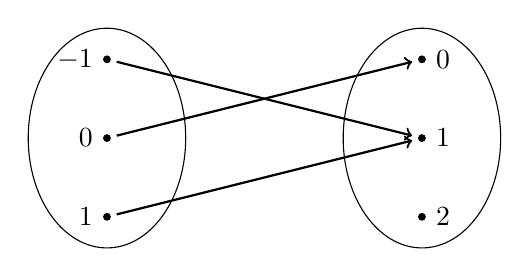
\begin{tikzpicture}[ele/.style={fill=black,circle,minimum width=.8pt,inner sep=1pt},every fit/.style={ellipse,draw,inner sep=-2pt}]
  \usetikzlibrary{fit}
  \node[ele,label=left:$-1$] (a2) at (0,3) {};    
  \node[ele,label=left:$0$] (a3) at (0,2) {};
  \node[ele,label=left:$1$] (a4) at (0,1) {};

  \node[ele,,label=right:$0$] (b2) at (4,3) {};
  \node[ele,,label=right:$1$] (b3) at (4,2) {};
  \node[ele,,label=right:$2$] (b4) at (4,1) {};

  \node[draw,fit= (a2) (a3) (a4),minimum width=2cm] {} ;
  \node[draw,fit=  (b2) (b3) (b4),minimum width=2cm] {} ;  
  \draw[->,thick,shorten <=2pt,shorten >=2] (a2) -- (b3);
  \draw[->,thick,shorten <=2pt,shorten >=2] (a3) -- (b2);
  \draw[->,thick,shorten <=2pt,shorten >=2] (a4) -- (b3);
 \end{tikzpicture}
\end{figure}

Every function say $f : A \rightarrow B$ satisfies the following conditions:\\
($i$) $f \subseteq A\times B$,   ($ii$) $\forall a\in A \Rightarrow (a, f(a)) \in f$ and ($iii$) $(a, b)\in f\, \&\, (a, c) \in f \Rightarrow b = c$
\begin{example}
Which of the following correspondences can be called a function ?
\begin{align*}
&(a) f(x) = x^3 ;&\, &\{-1, 0, 1\} \rightarrow \{0, 1, 2, 3\}\\
&(b) f(x) = \pm \sqrt{x} ;&\, &\{0, 1, 4\} \rightarrow \{-2, -1, 0, 1, 2\}\\
&(c) f(x) = \sqrt{x} ;&\, &\{0, 1, 4\} \rightarrow \{-2, -1, 0, 1, 2\}\\
&(d) f(x) = -\sqrt{x} ;&\, &\{0, 1, 4\} \rightarrow \{-2, -1, 0, 1, 2\}
\end{align*}
\end{example}

\begin{soln}
$f(x)$ in ($c$) \& ($d$) are functions as definition of function is satisfied. while in case of ($a$) the given relation is not a function, as $f(-1) \not\in $ codomain. Hence definition of function is not satisfied. While in case of ($b$), the given relation is not a function, as $f(1) = \pm 1$ and $f(4) = \pm 2$, $i.e.$ element 1 as well as 4 in domain is related with two elements of codomain. Hence definition of function is not satisfied
\end{soln}
\begin{example}
Which of the following pictorial diagrams represent the function?\\

 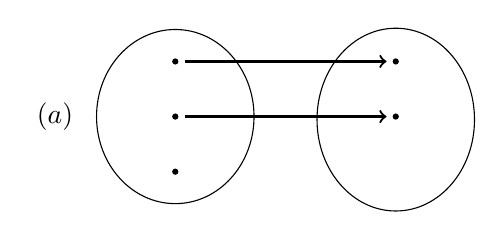
\begin{tikzpicture}[ele/.style={fill=black,circle,minimum width=.4pt,inner sep=.8pt},every fit/.style={ellipse,draw,inner sep=1pt},scale=0.7]
  \usetikzlibrary{fit}
  \node[label=left:$(a)$] (a5) at (-1.5,2) {};    
  \node[ele,label=left:] (a2) at (0,3) {};    
  \node[ele,label=left:] (a3) at (0,2) {};
  \node[ele,label=left:] (a4) at (0,1) {};

  \node[ele,,label=right:] (b2) at (4,3) {};
  \node[ele,,label=right:] (b3) at (4,2) {};
  \node[label=right:] (b4) at (4,1) {};

  \node[draw,fit= (a2) (a3) (a4),minimum width=2cm] {} ;
  \node[draw,fit=  (b2) (b3) (b4),minimum width=2cm] {} ;  
  \draw[->,thick,shorten <=2pt,shorten >=2] (a2) -- (b2);
  \draw[->,thick,shorten <=2pt,shorten >=2] (a3) -- (b3);
 \end{tikzpicture}
 \qquad
  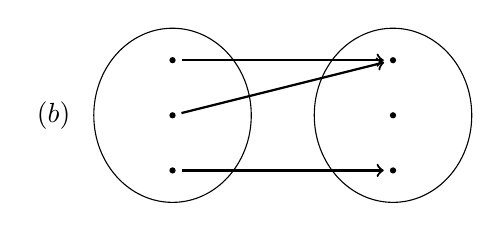
\begin{tikzpicture}[ele/.style={fill=black,circle,minimum width=.4pt,inner sep=.8pt},every fit/.style={ellipse,draw,inner sep=1pt},scale=0.7]
  \usetikzlibrary{fit}
  \node[label=left:$(b)$] (a5) at (-1.5,2) {};    
  \node[ele,label=left:] (a2) at (0,3) {};    
  \node[ele,label=left:] (a3) at (0,2) {};
  \node[ele,label=left:] (a4) at (0,1) {};

  \node[ele,,label=right:] (b2) at (4,3) {};
  \node[ele,,label=right:] (b3) at (4,2) {};
  \node[ele,,label=right:] (b4) at (4,1) {};

  \node[draw,fit= (a2) (a3) (a4),minimum width=2cm] {} ;
  \node[draw,fit=  (b2) (b3) (b4),minimum width=2cm] {} ;  
  \draw[->,thick,shorten <=2pt,shorten >=2] (a2) -- (b2);
  \draw[->,thick,shorten <=2pt,shorten >=2] (a3) -- (b2);
  \draw[->,thick,shorten <=2pt,shorten >=2] (a4) -- (b4);
 \end{tikzpicture}\\
 
  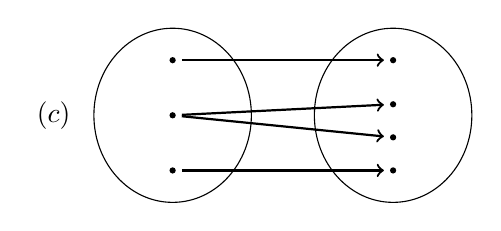
\begin{tikzpicture}[ele/.style={fill=black,circle,minimum width=.4pt,inner sep=.8pt},every fit/.style={ellipse,draw,inner sep=1pt},scale=0.7]
  \usetikzlibrary{fit}
  \node[label=left:$(c)$] (a5) at (-1.5,2) {};    
  \node[ele,label=left:] (a2) at (0,3) {};    
  \node[ele,label=left:] (a3) at (0,2) {};
  \node[ele,label=left:] (a4) at (0,1) {};

  \node[ele,,label=right:] (b2) at (4,1) {};
  \node[ele,,label=right:] (b3) at (4,1.6) {};
  \node[ele,,label=right:] (b4) at (4,2.2) {};
  \node[ele,,label=right:] (b5) at (4,3) {};
  \node[draw,fit= (a2) (a3) (a4),minimum width=2cm] {} ;
  \node[draw,fit=  (b2) (b3) (b4)(b5),minimum width=2cm] {} ;  
  \draw[->,thick,shorten <=2pt,shorten >=2] (a4) -- (b2);
  \draw[->,thick,shorten <=2pt,shorten >=2] (a2) -- (b5);
  \draw[->,thick,shorten <=2pt,shorten >=2] (a3) -- (b3);
 \draw[->,thick,shorten <=2pt,shorten >=2] (a3) -- (b4);
 \end{tikzpicture}
 \qquad
  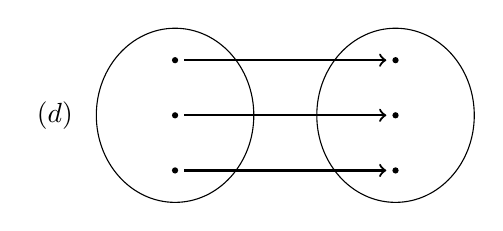
\begin{tikzpicture}[ele/.style={fill=black,circle,minimum width=.4pt,inner sep=.8pt},every fit/.style={ellipse,draw,inner sep=1pt},scale=0.7]
  \usetikzlibrary{fit}
  \node[label=left:$(d)$] (a5) at (-1.5,2) {};    
  \node[ele,label=left:] (a2) at (0,3) {};    
  \node[ele,label=left:] (a3) at (0,2) {};
  \node[ele,label=left:] (a4) at (0,1) {};

  \node[ele,,label=right:] (b2) at (4,3) {};
  \node[ele,,label=right:] (b3) at (4,2) {};
  \node[ele,,label=right:] (b4) at (4,1) {};

  \node[draw,fit= (a2) (a3) (a4),minimum width=2cm] {} ;
  \node[draw,fit=  (b2) (b3) (b4),minimum width=2cm] {} ;  
  \draw[->,thick,shorten <=2pt,shorten >=2] (a2) -- (b2);
  \draw[->,thick,shorten <=2pt,shorten >=2] (a3) -- (b3);
  \draw[->,thick,shorten <=2pt,shorten >=2] (a4) -- (b4);
 \end{tikzpicture}
\end{example}
\begin{soln}
$(b)$ \& $(d)$. In $(a)$ one element of domain has no image, while in $(c)$ one element of domain has two images
in codomain
\end{soln}
\begin{example}
Let $g(x)$ be a function defined on $[-1, 1]$. If the area of the equilateral triangle with two of its vertices at $(0,0)$ \& $(x,g(x))$ is $\dfrac{3}{4}$ sq.units, then the function $g(x)$ may be-\\
$(a)\, g(x)=\pm\sqrt{1-x^2}$\qquad $(b)\, g(x)=\sqrt{1-x^2}$\qquad $(c)\, g(x)=-\sqrt{1-x^2}$\qquad $(d)\, g(x)=\sqrt{1+x^2}$
\end{example}
\begin{soln}
Answer is $(b)$.
\end{soln}
\begin{example}
Represent all possible functions defined from $\{\alpha, \beta\}$ to $\{1, 2\}$.
\end{example}

\begin{soln}

  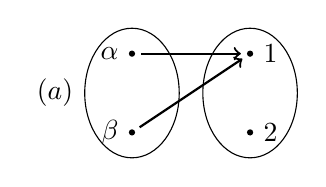
\begin{tikzpicture}[ele/.style={fill=black,circle,minimum width=.4pt,inner sep=.8pt},every fit/.style={ellipse,draw,inner sep=1pt}]
  \usetikzlibrary{fit}
  \node[label=left:$(a)$] (a5) at (-.5,1.5) {};    
  \node[ele,label=left:$\alpha$] (a3) at (0,2) {};
  \node[ele,label=left:$\beta$] (a4) at (0,1) {};

  \node[ele,,label=right:$1$] (b3) at (1.5,2) {};
  \node[ele,,label=right:$2$] (b4) at (1.5,1) {};

  \node[draw,fit= (a3) (a4),minimum width=1.2cm] {} ;
  \node[draw,fit=  (b3) (b4),minimum width=1.2cm] {} ;  
  \draw[->,thick,shorten <=2pt,shorten >=2] (a3) -- (b3);
  \draw[->,thick,shorten <=2pt,shorten >=2] (a4) -- (b3);
 \end{tikzpicture}
 \quad
   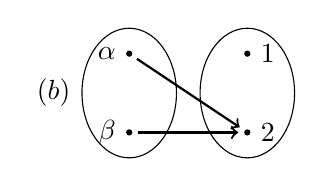
\begin{tikzpicture}[ele/.style={fill=black,circle,minimum width=.4pt,inner sep=.8pt},every fit/.style={ellipse,draw,inner sep=1pt}]
  \usetikzlibrary{fit}
  \node[label=left:$(b)$] (a5) at (-.5,1.5) {};    
  \node[ele,label=left:$\alpha$] (a3) at (0,2) {};
  \node[ele,label=left:$\beta$] (a4) at (0,1) {};

  \node[ele,,label=right:$1$] (b3) at (1.5,2) {};
  \node[ele,,label=right:$2$] (b4) at (1.5,1) {};

  \node[draw,fit= (a3) (a4),minimum width=1.2cm] {} ;
  \node[draw,fit=  (b3) (b4),minimum width=1.2cm] {} ;  
  \draw[->,thick,shorten <=2pt,shorten >=2] (a3) -- (b4);
  \draw[->,thick,shorten <=2pt,shorten >=2] (a4) -- (b4);
 \end{tikzpicture}
 \quad
   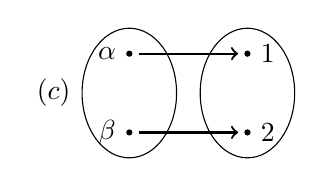
\begin{tikzpicture}[ele/.style={fill=black,circle,minimum width=.4pt,inner sep=.8pt},every fit/.style={ellipse,draw,inner sep=1pt}]
  \usetikzlibrary{fit}
  \node[label=left:$(c)$] (a5) at (-.5,1.5) {};    
  \node[ele,label=left:$\alpha$] (a3) at (0,2) {};
  \node[ele,label=left:$\beta$] (a4) at (0,1) {};

  \node[ele,,label=right:$1$] (b3) at (1.5,2) {};
  \node[ele,,label=right:$2$] (b4) at (1.5,1) {};

  \node[draw,fit= (a3) (a4),minimum width=1.2cm] {} ;
  \node[draw,fit=  (b3) (b4),minimum width=1.2cm] {} ;  
  \draw[->,thick,shorten <=2pt,shorten >=2] (a3) -- (b3);
  \draw[->,thick,shorten <=2pt,shorten >=2] (a4) -- (b4);
 \end{tikzpicture}
 \quad
   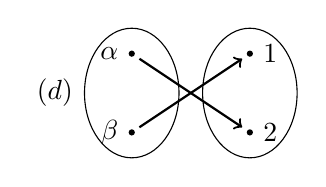
\begin{tikzpicture}[ele/.style={fill=black,circle,minimum width=.4pt,inner sep=.8pt},every fit/.style={ellipse,draw,inner sep=1pt}]
  \usetikzlibrary{fit}
  \node[label=left:$(d)$] (a5) at (-.5,1.5) {};    
  \node[ele,label=left:$\alpha$] (a3) at (0,2) {};
  \node[ele,label=left:$\beta$] (a4) at (0,1) {};

  \node[ele,,label=right:$1$] (b3) at (1.5,2) {};
  \node[ele,,label=right:$2$] (b4) at (1.5,1) {};

  \node[draw,fit= (a3) (a4),minimum width=1.2cm] {} ;
  \node[draw,fit=  (b3) (b4),minimum width=1.2cm] {} ;  
  \draw[->,thick,shorten <=2pt,shorten >=2] (a3) -- (b4);
  \draw[->,thick,shorten <=2pt,shorten >=2] (a4) -- (b3);
 \end{tikzpicture}
\end{soln}
\section{Domain, Co-domain \& Range of a Function :}
Let $f: A \rightarrow B$, then the set $A$ is known as the domain of $f$ \& the set $B$ is known as co-domain of $f$. If a member $'a'$ of $A$ is associated to the member $'b'$ of $B$, then $'b'$ is called the \textbf{$f-$image} of $'a'$ and we write $b = f (a)$. Further $'a'$ is called a pre-image of $'b'$. The set $\{f(a): \forall a \in A\}$ is called the range of $f$ and is denoted by $f(A)$. Clearly $f(A) \subseteq B$.\\
Sometimes if only definition of $f (x)$ is given (domain and codomain are not mentioned), then domain is set of those values of $'x'$ for which $f (x)$ is defined, while codomain is considered to be $(-\infty, \infty)$
A function whose domain and range both are sets of real numbers is called a \textbf{real function}. Conventionally the word \say{$FUNCTION$} is used only as the meaning of real function.
\begin{example}
Find the domain of following functions :$(i)\quad f(x)= \sqrt{x^2 -5}\qquad (ii)\quad f(x) = \sin^{-1}(2x-1)$
\end{example}
\begin{soln}

$(i)\quad f(x)= \sqrt{x^2 -5}$ is real iff $x^{2}-5\ge 0\, \Rightarrow |x|\ge \sqrt{5}\,\Rightarrow x\le \sqrt{5}\; or\; x\ge \sqrt{5}$\\ $\therefore$ The domain of $f$ is $(-\infty, -\sqrt{5}]\cup [\sqrt{5},\infty)\quad(ii)\quad  -1 \le 2x-1 \le 1\quad \therefore$ domain is $x \in [0, 1]$
\end{soln}
\subsection{Algebraic Operations on Functions :}
If $f$ \& $g$ are real valued functions of $x$ with domain set $A$ and $B$ respectively, then both $f$ \& $g$ are defined in $A \cap B$.
Now we define $(f + g)$, $(f-g)$, $(f\cdot g)$ \& $\Bigg(\dfrac{f}{g}\Bigg)$ as follows:
\begin{align*}
   \left.\begin{array}{rl}
        & (i)\; (f\pm g)(x) = f(x)\pm g(x)\\
        & (ii)\; (f\cdot g) = f(x)\cdot g(x)\\
           \end{array}
        \right\} domain\;in\;each\;case\;is\;A\cap B 
\end{align*}
\[\quad\;\,(iii)\Bigg(\dfrac{f}{g}\Bigg)(x)= \dfrac{f(x)}{g(x)}\quad \textit{domain is }\{x|x\in A\cap B \textit{such that }\; g(x)\neq 0 \} \]
$\bigstar$ For domain of $\phi(x) = \{f(x)\}^{g(x)}$ , conventionally, the conditions are $f(x) > 0$ and $g(x)$ must be defined.\\
$\bigstar$ For domain of $\phi(x) = \comb[f(x)]{g(x)}$ or $\phi(x) =\perm[f(x)]{g(x)}$ conditions of domain are $f(x)\ge g(x)$ and $f(x)\in \mathbb{N}$ and $g(x) \in \mathbb{N}$ 
\begin{example}
Find the domain of the following functions: \\
$(i)\;f(x)=\sqrt{\sin x}-\sqrt{16-x^2}\quad (ii)\;f(x)=\dfrac{3}{\sqrt{4-x^2}}\log(x^{3}-x)\quad (iii)\;f(x)=x^{\cos^{-1}x}$
\end{example}
\begin{soln}
$(i)\,\sqrt{\sin x}$ is real iff $\sin x \ge 0\Longleftrightarrow x\in [2n\pi, (2n +1)\pi],\;n\in \mathbb{Z}$\\$\sqrt{16-x^2}$ is real iff  $16-x^2 \ge 0 \Longleftrightarrow -4\le x\le 4$\\
Thus the domain of the given function is $ \{x : x\in[2n\pi, (2n+1)\pi],\; n\in\mathbb{Z}\}\cap[-4, 4] = [-4,-\pi] \cup [0, \pi]$\\
$(ii)$ Domain of of $\sqrt{4-x^2}$ is $[-2,2]$ but here $\sqrt{4-x^2} \neq 0 \therefore x\neq \pm 2 \Rightarrow x\in (-2,2)$ again $\log(x^3 -x)$ is defined for $x^3 -x >0\; i.e\; x(x+1)(x-1)>0 \quad \therefore$  The domain of  $\log(x^3 -x)$ is $(-1,0)\cup (1,\infty)$\\
Hence the domain of given function is $\{ (-1,0)\cup (1,\infty)\}\cap (-2,2) = (-1,0)\cup (1,2)$.\\
$(iii)\; x>0\; and\;  -1\le x\le 1\qquad \therefore$ domain is $(0,1]$ 
\end{soln}
\textbf{Assignment:} Find the domain of the following functions:\\
$(i)\; f(x)=\dfrac{1}{\log(2-x)} +\sqrt{x+1}\qquad (ii)\; f(x) = \sqrt{1-x}-\sin^{-1}\dfrac{2x-1}{3}$\\
\textbf{Answers:} $(i)\; [-1,1)\cup (1,2)\quad (ii)\; [-1,1] $
\subsection{Method of determining range:}
\subsection*{Representing $x$ in terms of $y$}Definition of the function is usually represented as $y\; (i.e. f(x)$ which is dependent variable) in terms of an expression of $x$ (which is independent variable). To find range rewrite given definition so as to represent $x$ in terms of an expression of $y$ and thus obtain range (possible values of $y$).
If $y = f(x)\Longleftrightarrow  x = g(y)$, then domain of $g(y)$ represents possible values of $y,\; i.e$. range of $f(x)$.
\begin{example}
Find the range of $f(x) = \dfrac{x^2+x+1}{x^2+x-1}$
\end{example}
\begin{soln}
$f(x) = \dfrac{x^2+x+1}{x^2+x-1}$ where $x^2+x+1$ and $x^2+x-1$ have no common factor.\\
Let, $y = \dfrac{x^2+x+1}{x^2+x-1}\Rightarrow yx^2+yx-y = x^2+x+1 \Rightarrow (y-1)x^{2}+(y-1)x -y-1=0$  if $y=1$ then the equation reduces to $-2=0$ which is not true. Further if $y\neq 1$ then $(y-1)x^{2}+(y-1)x -y-1=0$ is quadratic and has real roots if $(y-1)^{2}-4(y-1)(-y-1)\ge 0\quad \therefore$ if $y\le -\dfrac{3}{5}\; or\; y\ge 1$ but $y\neq 1.$ \\ Thus the range of the given function is $(-\infty,-\dfrac{3}{5}]\cup (1,\infty)$
\end{soln}
\subsection*{Graphical Method}
Values covered on $y-axis$ by the graph of function is range
\begin{example}
Find the range of $f(x) = \dfrac{x^2-4}{x-2}$
\end{example}
\begin{soln}
$ f(x) =\dfrac{x^2 -4}{x-2} = x+2;\; x\neq 2 $\\
$\therefore$ The graph of $f(x)$ would be:
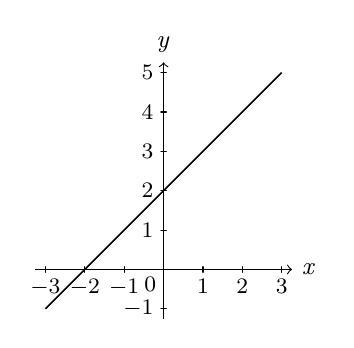
\begin{tikzpicture}[scale=.5]
\datavisualization [school book axes,
                    visualize as smooth line,
                    y axis={label},
                    x axis={label} ]

data [format=function] {
      var x : interval [-3:3] samples 150;
      func y =  \value x + 2 ;
      };
\end{tikzpicture}

\end{soln}
\end{document}